% ===================== TrajErrBench =====================
\subsection{TrajErrBench (TrajDebug)}\label{ds:trajerrbench}
\badgerow{\naturalbadge\ \okbadge\ \lbl{step + module.subtype}\ \lbl{single-agent}\ \lbl{$\tau^2$-Bench airline / retail \textperiodcentered\ SWE-Bench Pro}}

\begin{identity}
Paper & \emph{TrajDebug: Tracing Error Lifecycle to Identify Critical Failures in Long-Horizon Agent Trajectories} --- Qi, Yin, Shi, Peng, Lu, Liu, Xuan, Liu, Hu, Wang, Hou, Xu, Li (Tsinghua THU-KEG, with industry co-authors), Findings of EMNLP 2026 (accepted 2026-08-20), arXiv:2608.06346 \cite{trajdebug2026}\\
Links & \href{https://github.com/THU-KEG/TrajDebug}{GitHub \code{THU-KEG/TrajDebug}} (code + \code{data/trajerrbench/\{en,zh\}}; English edition released 2026-09-07; the repo also ships Who\&When and AgentErrorBench converted to the same schema) \textperiodcentered\ no HF dataset\\
License & MIT for the TrajDebug code and annotations (\code{LICENSE}, \code{CITATION.cff}); task text and trajectories remain under $\tau^2$-Bench and SWE-Bench Pro terms (\code{data/README.md})\\
Status & downloaded in full (git clone), ungated; 486 zh + 486 en JSON files = 63 MB (clone 215 MB); \code{data/trajerrbench/repo\_TrajDebug/data/trajerrbench/\{en,zh\}/\{tau2bench,swebenchpro\}/*.json} + \code{manifest.jsonl}\\
\end{identity}

\begin{multicols}{2}
\paragraph{Description} TrajErrBench is a benchmark for \emph{critical error step detection} in long-horizon single-agent trajectories, using Who\&When's counterfactual definition: the critical step is the \emph{earliest} decisive error, i.e.\ the step whose action, if replaced by a correct one (earlier steps fixed, later steps unfolding correctly), would have turned the failure into a success. Detection uses the failed trajectory alone, without task ground truth. Failures are natural (reward 0 under the source benchmark's own evaluation). Two domains:
\begin{itemize}
\item \textbf{$\tau^2$-Bench} (400): airline and retail customer-service tool-use tasks with a simulated user; rollouts by DeepSeek-Reasoner, GPT-5 and Qwen3-Max; 29.3 messages on average.
\item \textbf{SWE-Bench Pro} (86): repository-level issue fixing in the OpenHands scaffold; rollouts by Claude-Opus-4.6, Kimi-K2.6-Coding, Gemini-3.1-Pro and Grok-4.20-Beta (GPT-5.4 is listed in the paper but absent from the released ids); 119.7 messages on average.
\end{itemize}
\textbf{Annotation}: GPT-5.4, Gemini-3.1-Pro and Claude-Opus-4.6 pre-annotate with the trajectory \emph{plus} the benchmark's failure diagnostics (unmet DB constraints / failing tests) as a reference; a pool of 20 trained annotators then labels \textbf{3 per trajectory}, and the majority ($\ge$2/3) is the label. Guideline: the step must contain an explicit, evidence-supported mistake; it must be failure-responsible (locally repaired mistakes excluded); if several, take the earliest. SWE-Bench Pro started with 110 runs, 24 without a 2-way agreement were dropped. Fleiss' $\kappa$ on the critical step: \textbf{0.91} on $\tau^2$-Bench (pairwise 91.2\%), \textbf{0.67} on SWE-Bench Pro (66.7\%); execution phase 0.73 / 0.42; contradiction reference category 0.41 / 0.38 (paper Table 5). Pre-annotation exact match with the final label: Gemini 76.8\%, Claude 64.5\%, GPT-5.4 53.2\% on $\tau^2$; 31.4 / 48.8 / 55.8\% on SWE-Pro. \textbf{Labels}: \code{critical\_error\_step} (0-based message index; 485 assistant messages and one tool message) and \code{critical\_error\_type} = \code{<module>.<subtype>} from a 5-module / 20-subtype taxonomy --- PLAN (BadDecomposition, WrongOrder, UnrealisticPlan, GoalDrift, OverExplore), REASON (WrongChoice: visible evidence ignored or misquoted; InvalidInference: evidence cited but conclusion over-reaches; MissingAssumptionCheck: claim with no evidence), ACT (WrongTool, ToolSchemaMismatch, WrongActionSequence, UnsafeOrForbiddenAction), OBS (MisreadOutput, IgnoreOutput, TimingIssue, GroundingFail), VERIFY (NoVerification, WrongVerification, PrematureTermination, InfiniteRetry); 17 records have \code{null} type. Annotators' explanations, the execution phase and the reference category are \emph{not} shipped.

\paragraph{Metrics and baselines} Exact-step accuracy, plus a relaxed window $[\mathrm{GT}{-}3, \mathrm{GT}]$ in Appendix E (scorer: \code{detector/score\_steps.py}); the paper evaluates on the \textbf{zh} edition. TrajDebug itself compresses the trajectory at several granularities, detects error triggers, classifies each as resolved or terminal and attributes among a candidate set. Step accuracy in \% (paper Table 1; direct prompting = best of seven LLMs and GPT-5.4; AEB = AgentErrorBench ALFWorld / GAIA / WebShop, W\&W = Who\&When Hand-Crafted / Alg.-Generated):

\begin{center}\footnotesize\setlength{\tabcolsep}{2pt}
\fitbox{\begin{tabular}{@{}lcccccc@{}}\toprule
Method & $\tau^2$ & SWE-Pro & W\&W H / A & AEB A / G / W & Avg\\\midrule
Direct (Gemini-3.1-Pro) & 52.5 & 17.4 & 20.7 / 46.8 & 19.0 / 30.6 / 32.0 & 31.3\\
Direct (GPT-5.4) & 41.5 & 10.5 & 13.8 / 28.6 & 11.0 / 20.4 / 14.0 & 20.0\\
AgentDebugger & 26.0 & 10.5 & 12.1 / 40.5 & 21.0 / 36.0 / 20.0 & 23.7\\
CHIEF & 26.8 & 2.3 & 19.0 / 41.3 & 6.0 / 26.0 / 10.0 & 18.8\\
AgentRx & 36.3 & 5.8 & 25.9 / 41.3 & 8.0 / 26.5 / 18.0 & 23.1\\
TrajDebug & \textbf{52.8} & \textbf{24.4} & 22.4 / \textbf{48.4} & \textbf{26.0} / \textbf{38.8} / 26.0 & \textbf{34.1}\\\bottomrule
\end{tabular}}
\end{center}
SWE-Bench Pro is by far the hardest split (best 24.4\%), consistent with its lower human agreement.

\paragraph{Schema} One JSON file per trajectory in the unified TrajDebug schema (\code{data\_processing/schema.py}): \code{messages} = list of \{\code{step} (0-based, = array index), \code{role} (\code{system} / \code{user} / \code{assistant} / \code{tool}), \code{name}, \code{content} (tool calls rendered as \code{[tool\_calls]\textbackslash n- fn(\{json\})}), \code{judgable} (may this step be the critical one), \code{compress\_role}\}; \code{metadata}: \code{dataset} = \code{trajerrbench}, \code{task\_id}, \code{task\_description}, \code{reward} (0), \code{annotation.\{critical\_error\_step, critical\_error\_type\}}, \code{extra.\{agent\_framework\_description, language, source\_benchmark, pair\_id\}}. \code{manifest.jsonl} pairs the zh and en files; labels and message counts are identical across editions (0 mismatches). The same folder layout holds the converted \code{whoandwhen/} (58 + 126) and \code{agentdebugbench/} (100 + 50 + 50) copies.
\end{multicols}

\paragraph{Statistics} computed from the downloaded English edition (identical labels to zh).\par\nobreak\vspace{1pt}
\noindent\begin{minipage}[t]{0.56\linewidth}\vspace{0pt}\small\setlength{\tabcolsep}{4pt}
\fitbox{\begin{tabular}{@{}lrrr@{}}\toprule
 & All & $\tau^2$-Bench & SWE-Pro\\\midrule
trajectories (all failed) & 486 & 400 & 86\\
generating models & 7 & 3 & 4\\
messages: mean / med. & 45.2 / 29 & 29.3 / 27 & 119.2 / 117\\
messages: min -- max & 7 -- 202 & 7 -- 202 & 58 -- 180\\
assistant steps: mean / med.\ (max) & 21.5 / 14 (101) & --- & ---\\
critical msg index: mean / med.\ (max) & 27.0 / 19 (160) & --- & ---\\
rel.\ critical position: mean / med. & 0.63 / 0.65 & 0.64 / 0.66 & 0.59 / 0.62\\
chars / trajectory: mean / med. & 52.6\,k / 20.9\,k & 20.6\,k / 19.7\,k & 201\,k / 182\,k\\\bottomrule
\end{tabular}}

\smallskip Subsets by domain and model: retail / DeepSeek-Reasoner 103, airline / Qwen3-Max 80, retail / GPT-5 76, airline / DeepSeek-Reasoner 71, airline / GPT-5 70; SWE-Pro: Gemini-3.1-Pro 28, Claude-Opus-4.6 21, Grok-4.20 21, Kimi-K2.6 16. Blamed module: reason 58.0\%, plan 14.4\%, obs 10.9\%, act 7.0\%, verify 6.2\%, null 3.5\%; on SWE-Pro \code{reason.WrongChoice} alone is 40.7\% and all OBS subtypes are absent. Critical steps sit mid-to-late: 13.5\% in the first 40\% of the run, 42\% between 0.6 and 0.8, 19.8\% in the last fifth.
\end{minipage}\hfill
\begin{minipage}[t]{0.42\linewidth}\vspace{0pt}
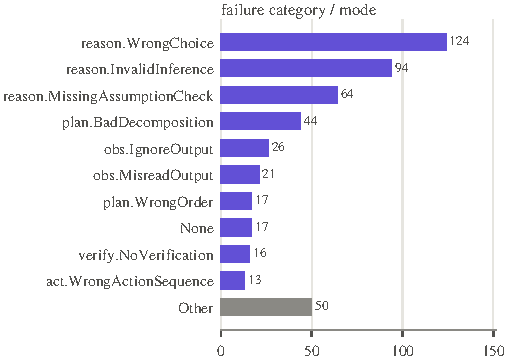
\includegraphics[width=\linewidth]{6_related/trajerrbench/figures/cat.pdf}
\end{minipage}

\paragraph{Example trajectory} \code{airline\_failed\_qwen3-max::0250f877-\dots} (en edition, $\tau^2$-Bench airline, Qwen3-Max; 7 messages, 8\,k characters --- the shortest $\tau^2$ run; step 0 is the airline policy prompt). The user asks for the balances of their gift cards and certificates; instead of identifying the user and looking up the account, the assistant immediately calls \code{transfer\_to\_human\_agents}, which ends the episode. Label: step 3, \code{act.WrongTool}; no free-text rationale is shipped.
% auto-generated by scripts/render_traj.py -- do not edit
\trajtask{airline\_failed\_qwen3-max:\allowbreak{}:\allowbreak{}0250f877-f44b-4ceb-990a-f284cc9c6433}{Hi,\allowbreak{} I'd like to check the balances on my gift cards and certificates,\allowbreak{} please. Could you let me know the total amounts I have for each?\allowbreak{}}
\begin{trajstep}{0}{system}{agA}
\# Airline Agent Policy\par The current time is 2024-05-15 15:\allowbreak{}00:\allowbreak{}00 EST.\par As an airline agent,\allowbreak{} you can help users **book**,\allowbreak{} **modify**,\allowbreak{} or **cancel** flight reservations. You also handle **refunds and compensation**.\par Before taking any actions that update the booking database (booking,\allowbreak{} modifying flights,\allowbreak{} editing baggage,\allowbreak{} changing cabin class,\allowbreak{} or updating passenger information),\allowbreak{} you must list the action details and obtain explicit user confirmation (yes) to proceed.\par You should not provide any information,\allowbreak{} knowledge,\allowbreak{} or procedures not provided by the user or available tools,\allowbreak{} or give subjective recommendations or comments.\par You should only make o\newline [...] (2,\allowbreak{}605 chars omitted) [...]\newline the agent can offer a certificate as a gesture after confirming the facts and changing or cancelling the reservation,\allowbreak{} with the amount being \$50 times the number of passengers.\par Do not offer compensation for any other reason than the ones listed above.
\end{trajstep}
\begin{trajstep}{1}{assistant}{agB}
Hi! How can I help you today?\allowbreak{}
\end{trajstep}
\begin{trajstep}{2}{user}{agC}
Hi,\allowbreak{} I'd like to check the balances on my gift cards and certificates,\allowbreak{} please. Could you let me know the total amounts I have for each?\allowbreak{}
\end{trajstep}
\begin{faultystep}{3}{assistant}{agB}
[tool\_calls]\newline - transfer\_to\_human\_agents(\{"summary":\allowbreak{} "User is requesting to check the balances on their gift cards and certificates,\allowbreak{} which is outside the scope of available tools and policy."\})
\end{faultystep}
\begin{trajstep}{4}{tool}{agD}
Transfer successful
\end{trajstep}
\begin{trajstep}{5}{assistant}{agB}
YOU ARE BEING TRANSFERRED TO A HUMAN AGENT. PLEASE HOLD ON.
\end{trajstep}
\begin{trajstep}{6}{user}{agC}
\#\#\#TRANSFER\#\#\#
\end{trajstep}
\trajannotation{assistant}{3}{act.WrongTool}{(no free-text rationale is shipped in the release;\allowbreak{} label =\allowbreak{} earliest failure-responsible step under the Who\&When decisive-error protocol)}{—}{YOU ARE BEING TRANSFERRED TO A HUMAN AGENT. PLEASE HOLD ON.}{\textbf{reward}: 0; \textbf{source\_benchmark}: tau2bench; \textbf{language}: en; \textbf{pair\_id}: tau2bench:\allowbreak{}airline\_failed\_qwen3-max:\allowbreak{}:\allowbreak{}0250f877-f44b-4ceb-990a-f284cc9c6433; \textbf{agent\_framework\_description}: A user interacts with a single `assistant` that must follow the scene policy shown in the leading `system` message while executing the user's request. `tool` messages are tool-call return values. Critical errors can only be attributed to an `assistant` step;\allowbreak{} `user` and `tool` steps are never the critical step. The assistant should try to fulfil the user's re\newline [...] (1,\allowbreak{}752 chars omitted) [...]\newline erified to be permitted commits the assistant to a path that may be unworkable,\allowbreak{} and the user may rely on the option as if it were available.}


\paragraph{Notes} (i) Closest to Who\&When's protocol (earliest decisive error, 3-way majority) but single-agent and long-horizon; it is the only set here with both a \emph{customer-service tool-use} domain (simulated user whose turns are never the critical step) and a \emph{coding} domain ($\approx$120 messages / 200\,k characters per run). (ii) Errors are mid-to-late (median relative position 0.65) because agents first gather information (dialogue, repo exploration) before the decisive decision --- the opposite of Failure-as-a-Process's early $t_{\mathrm{err}}$ (\S\ref{ds:failure_as_process}). (iii) Two language editions: the paper's numbers are on zh; en was built from aligned source trajectories and inherits the zh labels --- use en for English reports but cite results as zh. (iv) Missing from the release: annotator rationales, execution-phase and reference-category labels (aggregate only), the 24 dropped ambiguous SWE-Pro runs, and a type for 17 records. (v) Anchoring: annotators saw three LLM proposals \emph{and} the benchmark's failure diagnostics, whereas detectors see only the trajectory; the authors quantify this (Table 4) but it remains a caveat. (vi) Overlaps: ships converted Who\&When (\S\ref{ds:who_and_when}) and AgentErrorBench (\S\ref{ds:agenterrorbench}) copies --- a ready-made unified harness for all three --- and its taxonomy is a re-organisation of AgentDebug's five modules (plan / reason / act / obs / verify instead of memory / reflection / planning / action / system).
